\documentclass[tikz]{standalone}
\usepackage{pgfplots}
\pgfplotsset{compat=newest}
\pgfplotsset{every axis legend/.append style={%
cells={anchor=west}}
}
\usepgfplotslibrary{polar}
\usetikzlibrary{arrows}
\tikzset{>=stealth'}

\begin{document}
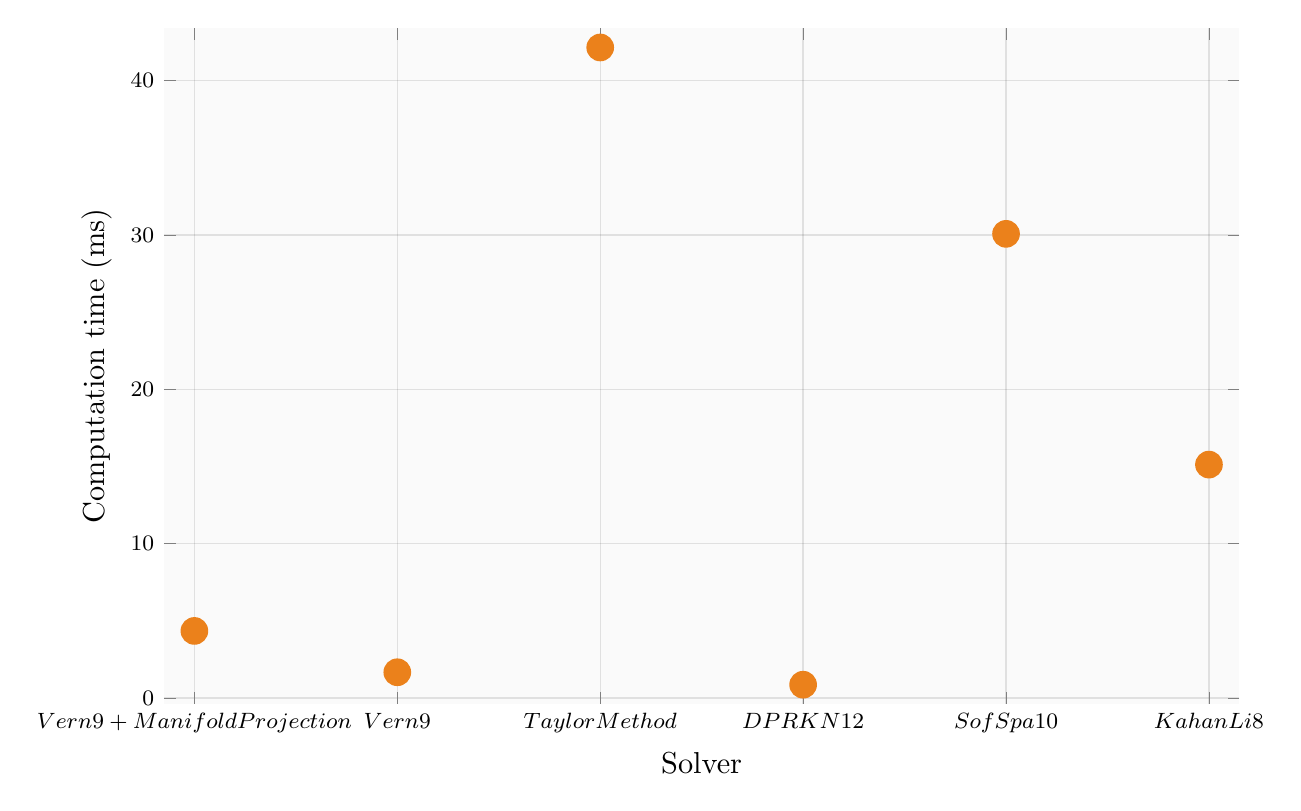
\begin{tikzpicture}[]
\begin{axis}[height = {101.6mm}, ylabel = {Computation time (ms)}, xmin = {0.35}, xmax = {5.65}, ymax = {43.382809030000004}, xlabel = {Solver}, unbounded coords=jump,scaled x ticks = false,xlabel style = {font = {\fontsize{11 pt}{14.3 pt}\selectfont}, color = {rgb,1:red,0.00000000;green,0.00000000;blue,0.00000000}, draw opacity = 1.0, rotate = 0.0},xmajorgrids = true,xtick = {0.5,1.5,2.5,3.5,4.5,5.5},xticklabels = {$Vern9+ManifoldProjection$,$Vern9$,$TaylorMethod$,$DPRKN12$,$SofSpa10$,$KahanLi8$},xtick align = inside,xticklabel style = {font = {\fontsize{8 pt}{10.4 pt}\selectfont}, color = {rgb,1:red,0.00000000;green,0.00000000;blue,0.00000000}, draw opacity = 1.0, rotate = 0.0},x grid style = {color = {rgb,1:red,0.00000000;green,0.00000000;blue,0.00000000},
draw opacity = 0.1,
line width = 0.5,
solid},x axis line style = {draw opacity = 0},scaled y ticks = false,ylabel style = {font = {\fontsize{11 pt}{14.3 pt}\selectfont}, color = {rgb,1:red,0.00000000;green,0.00000000;blue,0.00000000}, draw opacity = 1.0, rotate = 0.0},ymajorgrids = true,ytick = {0.0,10.0,20.0,30.0,40.0},yticklabels = {$0$,$10$,$20$,$30$,$40$},ytick align = inside,yticklabel style = {font = {\fontsize{8 pt}{10.4 pt}\selectfont}, color = {rgb,1:red,0.00000000;green,0.00000000;blue,0.00000000}, draw opacity = 1.0, rotate = 0.0},y grid style = {color = {rgb,1:red,0.00000000;green,0.00000000;blue,0.00000000},
draw opacity = 0.1,
line width = 0.5,
solid},y axis line style = {draw opacity = 0},    xshift = 0.0mm,
    yshift = 0.0mm,
    axis background/.style={fill={rgb,1:red,0.98039216;green,0.98039216;blue,0.98039216}}
,legend style = {color = {rgb,1:red,0.00000000;green,0.00000000;blue,0.00000000},
draw opacity = 1.0,
line width = 1,
solid,fill = {rgb,1:red,0.98039216;green,0.98039216;blue,0.98039216},font = {\fontsize{8 pt}{10.4 pt}\selectfont}},colorbar style={title=}, ymin = {-0.3849100299999999}, width = {152.4mm}]\addplot+[draw=none, color = {rgb,1:red,0.92156863;green,0.50588235;blue,0.10588235},
draw opacity = 1.0,
line width = 0,
solid,mark = *,
mark size = 5.0,
mark options = {
    color = {rgb,1:red,0.00000000;green,0.00000000;blue,0.00000000}, draw opacity = 0.0,
    fill = {rgb,1:red,0.92156863;green,0.50588235;blue,0.10588235}, fill opacity = 1.0,
    line width = 0,
    rotate = 0,
    solid
},forget plot] coordinates {
(0.5, 4.338601)
(1.5, 1.6609)
(2.5, 42.1441)
(3.5, 0.853799)
(4.5, 30.067001)
(5.5, 15.1162)
};
\end{axis}

\end{tikzpicture}
\end{document}
